\documentclass{beamer}

\usepackage[utf8x]{inputenc}
\usepackage{default}
\usetheme{PaloAlto}
\usecolortheme{seahorse}

\title{Sistemas Digitais 2\\ \textbf{Análise de FSM}}
\date{Brasíla, 02/2011}
\institute{\textbf{Universidade de Brasília - Faculdade do Gama}} 

\begin{document}

%SLIDE INICIAL DE APRESENTAÇÃO
\begin{frame}
  \titlepage
\end{frame}
  
%SEÇÃO == INTRODUÇÃO
\section{Introdução}Introdução
  \begin{frame}
    \frametitle{Introdução}
    \begin{itemize}
      \item Suponha que queiramos que um dado circuito sequencial realize cinco operações distintas onde cada operação representará um estado, 
	    portanto teremos cinco estados (um para cada opção). Além disto cada operação pode ser realizada milhares de vezes. \pause
      \item Outra característica deste circuito é que ele mesmo é responsável por ir de um estado atual para o próximo, ou seja, ele muda para 
	    o próximo estado lógico do circuito (next-state logic circuit).\pause
      \item O próximo estado nada mais é que um circuito combinacional que recebe o conteúdo de um estado da memória e as entradas atuais.\pause
      \item As saídas do próximo estado lógico, são usados para mudar o conteúdo do estado da memória (flip-flops). O circuito muda de estado quando 
	    o conteúdo da memória de estado muda.
    \end{itemize}
  \end{frame}

  \begin{frame}
    \frametitle{Introdução}
    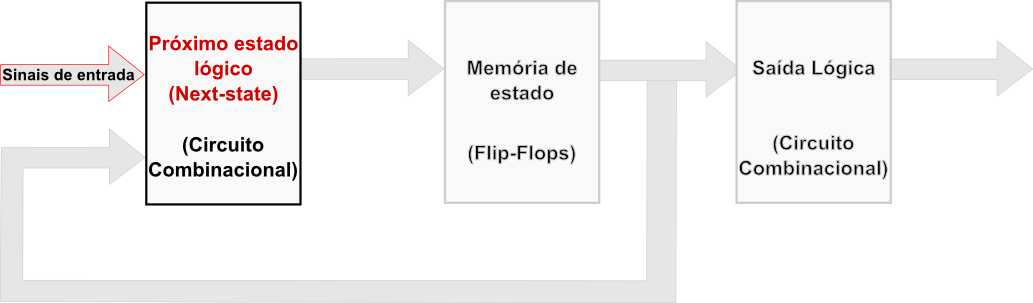
\includegraphics[height=1.3in, width=4in]{modelo_1.png}
  \end{frame}

  \begin{frame}
    \frametitle{Introdução}
    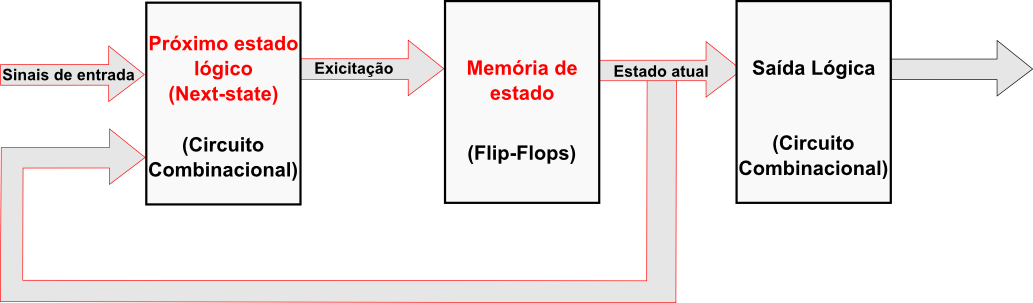
\includegraphics[height = 1.3in, width = 4in]{modelo_2.png}
  \end{frame}

  \begin{frame}
    \frametitle{Introdução}
    As saídas são dependentes do estado anterior, desta forma um estado é usado para lembrar as entradas anteriores e também determinar as saídas geradas. 
    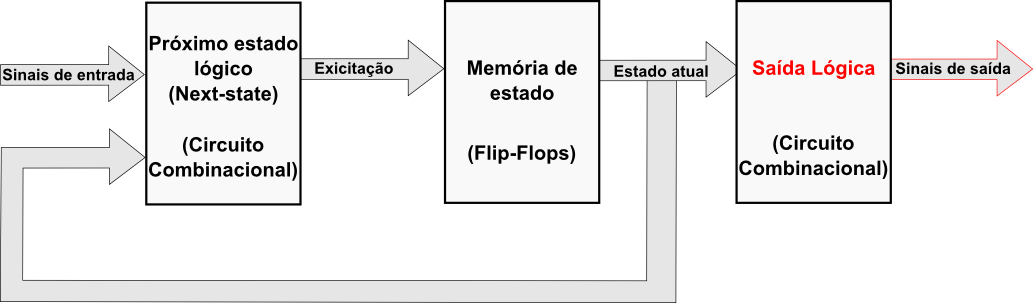
\includegraphics[height = 1.3in, width = 4in]{modelo_3.png}
  \end{frame}

  \begin{frame}
    \frametitle{Introdução}
    \begin{itemize}
      \item Um circuito sequencial também é conhecido por máquina de estados finitos (finite-state machine FSM), devido ao tamanho da memória ser finita, 
	    portanto o número de diferentes estados também é finito.\pause
      \item Este tipo de circuito é utilizado em projetos de unidades de controle, devido a sua flexibilidade e a possibilidade de haver várias saídas.
    \end{itemize}
  \end{frame}

%SEÇÃO == MODELOS DE FSM
\section{Modelos de FSM}
\begin{frame}
  \frametitle{Modelos de Máquina de Estados Finitas}
   Toda máquina de estado possuí três estruturas básicas, são elas:
\end{frame}

\begin{frame}
  \frametitle{Modelos de Máquina de Estados Finitas}
    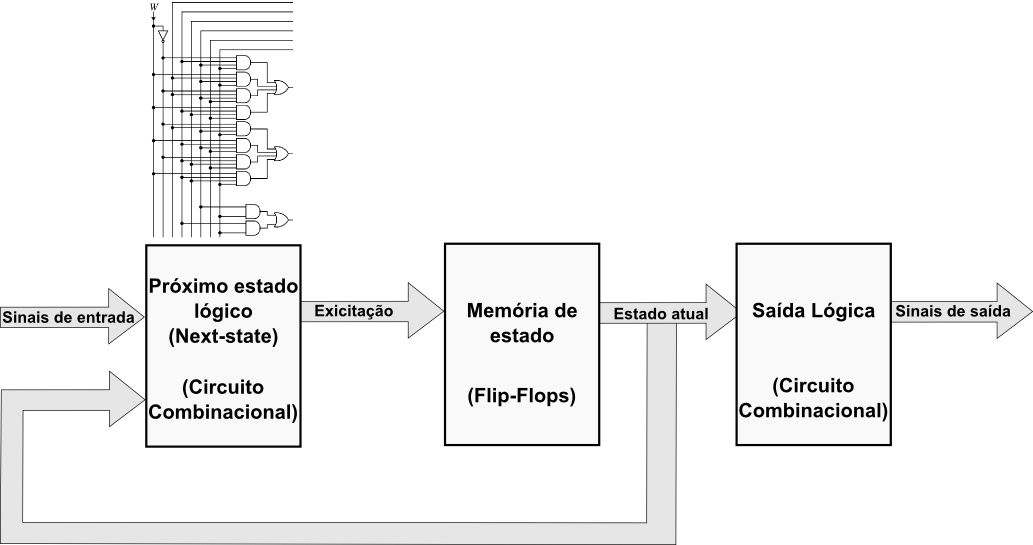
\includegraphics[height = 2.5in, width = 4in]{modelo_4.png}
\end{frame}

\begin{frame}
  \frametitle{Modelos de Máquina de Estados Finitas}
    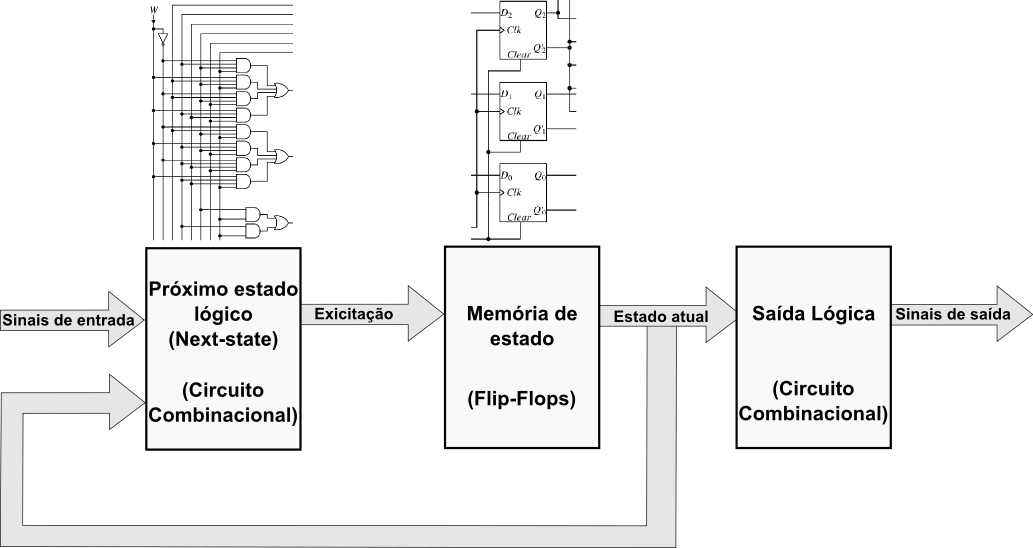
\includegraphics[height = 2in.5, width = 4in]{modelo_5.png}
\end{frame}

\begin{frame}
  \frametitle{Modelos de Máquina de Estados Finitas}
    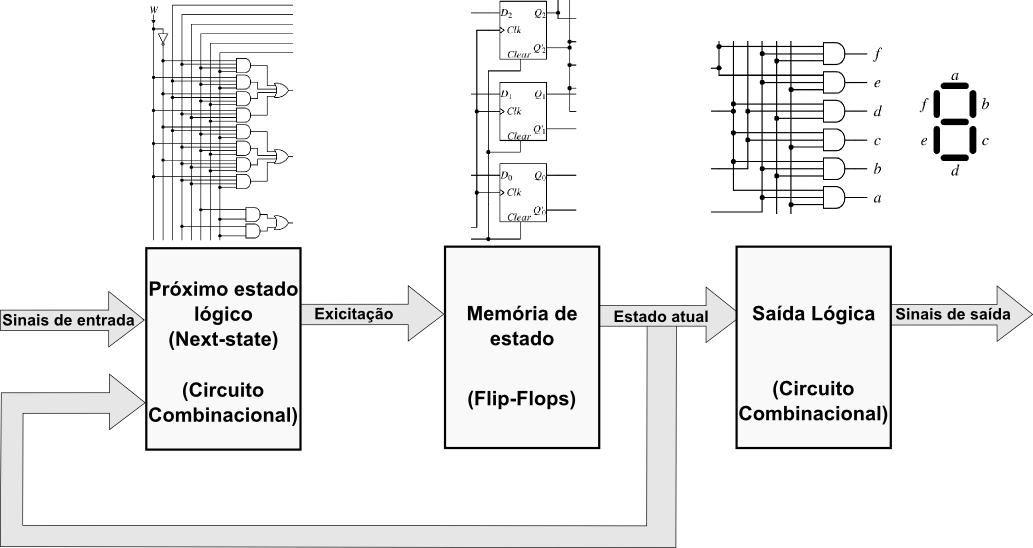
\includegraphics[height = 2.5in, width = 4in]{modelo_6.png}
\end{frame}

\begin{frame}
  \frametitle{Modelos de Máquina de Estados Finitas}
  \begin{itemize}
    \item A saída em uma máquina de estados pode ou não depender da entrada, com isto podemos definir o dois modelos: Moore e o Mealy.\pause
    \item Tanto as máquinas Moore e Mealy a única diferença entre os dois esta na forma como a saída é gerada.
  \end{itemize}
\end{frame}

\begin{frame}
  \frametitle{Modelos de Máquina de Estados Finitas}
    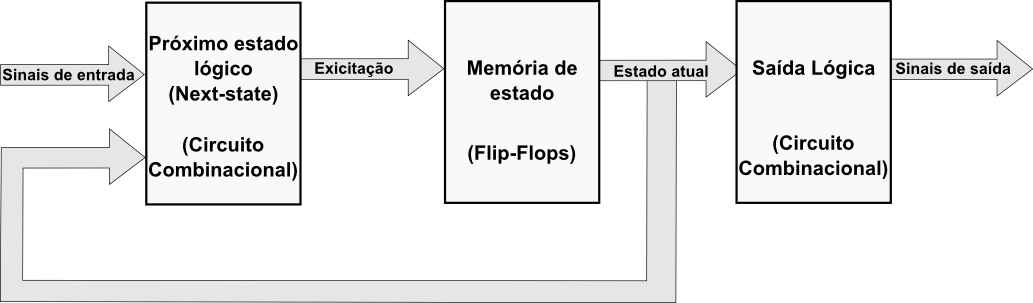
\includegraphics[height = 1.3in, width = 4in]{modelo_7.png}
\end{frame}

\begin{frame}
  \frametitle{Modelos de Máquina de Estados Finitas}
    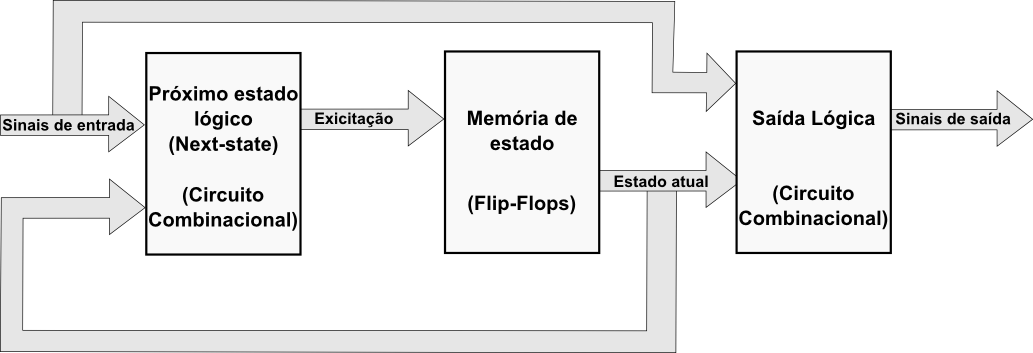
\includegraphics[height = 1.3in, width = 4in]{modelo_8.png}
\end{frame}

\begin{frame}
  \frametitle{Modelos de Máquina de Estados Finitas}
  \textbf{Deve-se ficar bem claro que ambas as máquinas são idênticas diferenciando-se somente na forma como a saída é produzida.}
\end{frame}


%SEÇÃO == DIAGRAMA DE ESTADOS
\section{Diagrama de estados}
\begin{frame}
  \frametitle{Diagrama de estados}
  \begin{itemize}
    \item Descrevem as operações de uma máquina de estados finita.\pause
    \item Cada estado existente é representado por um nó e este nó é rotulado por um nome ou um código.\pause
    \item Para toda transição de estado da FSM, cada nó é conectador por uma linha, que pode ser rotulada ou não. Os rótulos indicam duas características:\pause
    \begin{enumerate}
     \item Linhas rotuladas indicam \textbf{condições} para uma transição.\pause
     \item Linhas sem rótulos indicam transições \textbf{incondicionais}. Neste caso \textit{somente} uma linha incondicional pode ser originada por estado.\pause
    \end{enumerate}
    \item Por uma questão de clareza entre os modelos adota-se a seguinte diferenciação no diagrama de estados:\pause
    \begin{enumerate}
     \item Moore: A saída é colocada dentro do estado.\pause
     \item Mealy: A saída é colocada sobre as linhas que indicam a transição.
    \end{enumerate}
  \end{itemize}
\end{frame}

\begin{frame}
  \frametitle{Diagrama de estados}
    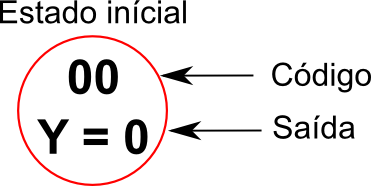
\includegraphics[height = 1.7in, width = 3.5in]{mealyvsmoore.png}
\end{frame}

\begin{frame}
  \frametitle{Diagrama de estados}
    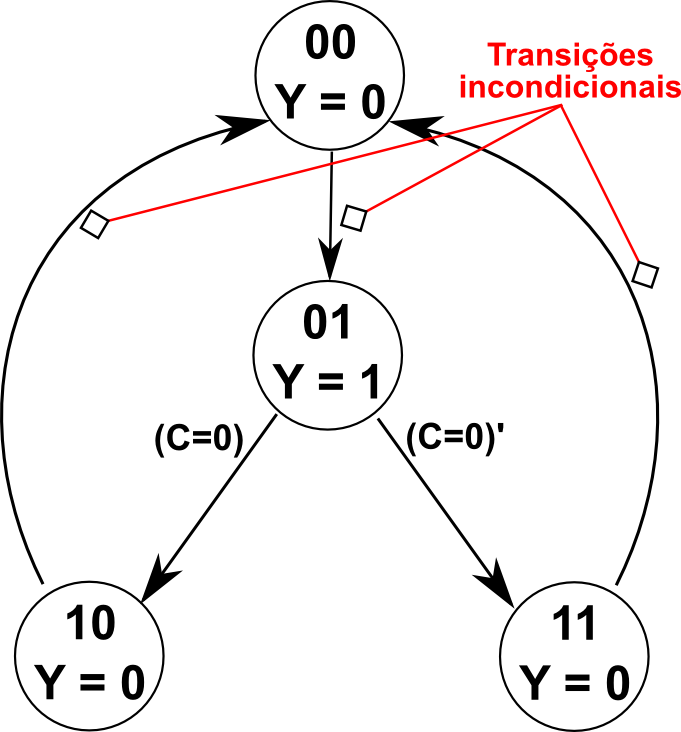
\includegraphics[height = 2.5in, width = 3in]{mealyvsmoore_2.png}
\end{frame}

\begin{frame}
  \frametitle{Diagrama de estados}
    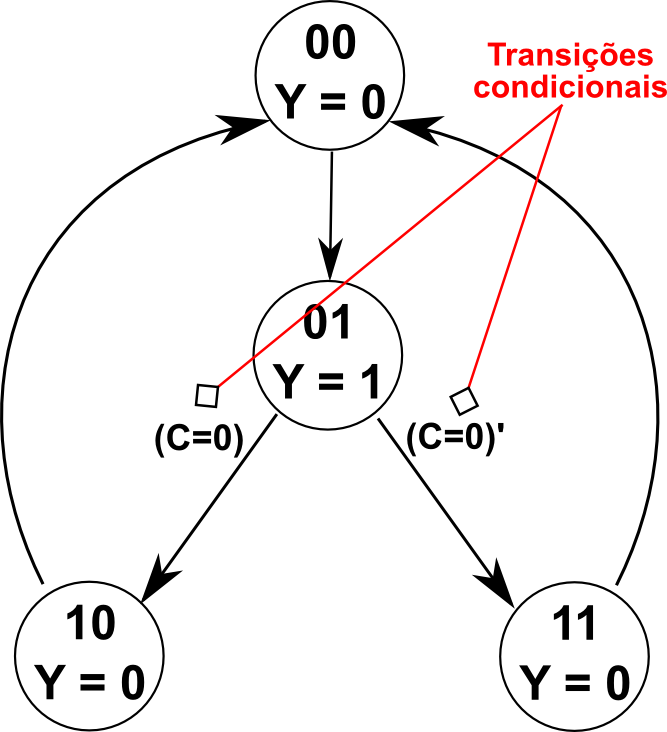
\includegraphics[height = 2.5in, width = 3in]{mealyvsmoore_3.png}
\end{frame}

\begin{frame}
  \frametitle{Diagrama de estados}
    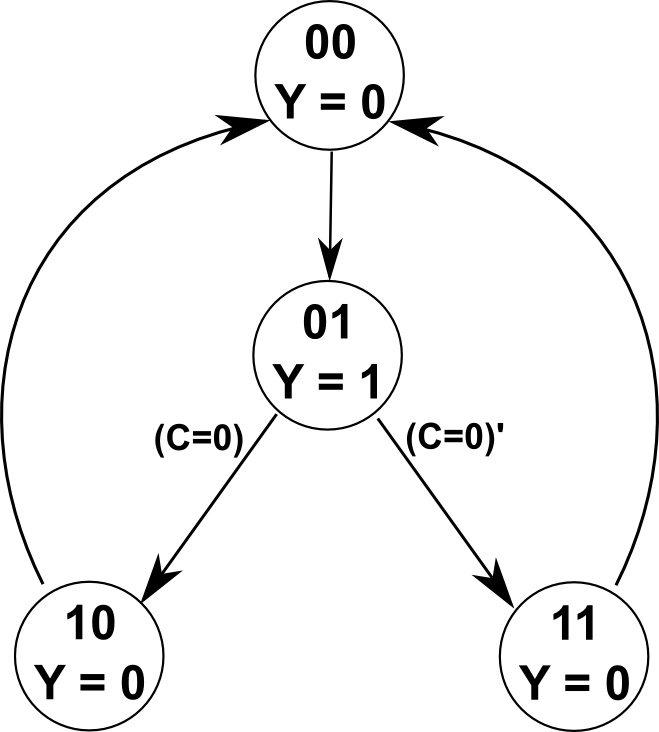
\includegraphics[height = 2.5in, width = 3in]{mealyvsmoore_4.png}
\end{frame}

\begin{frame}
  \frametitle{Diagrama de estados}
    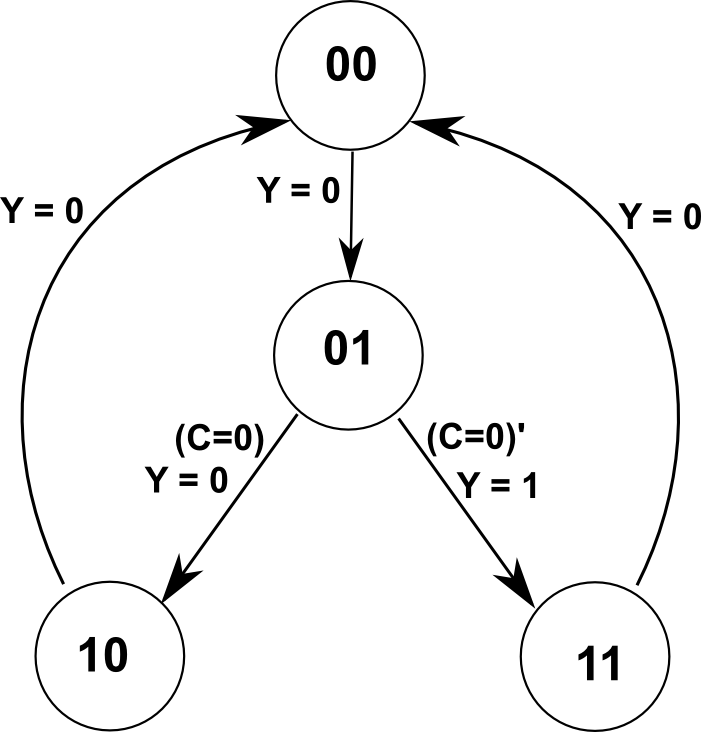
\includegraphics[height = 2.5in, width = 3in]{mealyvsmoore_5.png}
\end{frame}

\begin{frame}
  \frametitle{Diagrama de estados}
    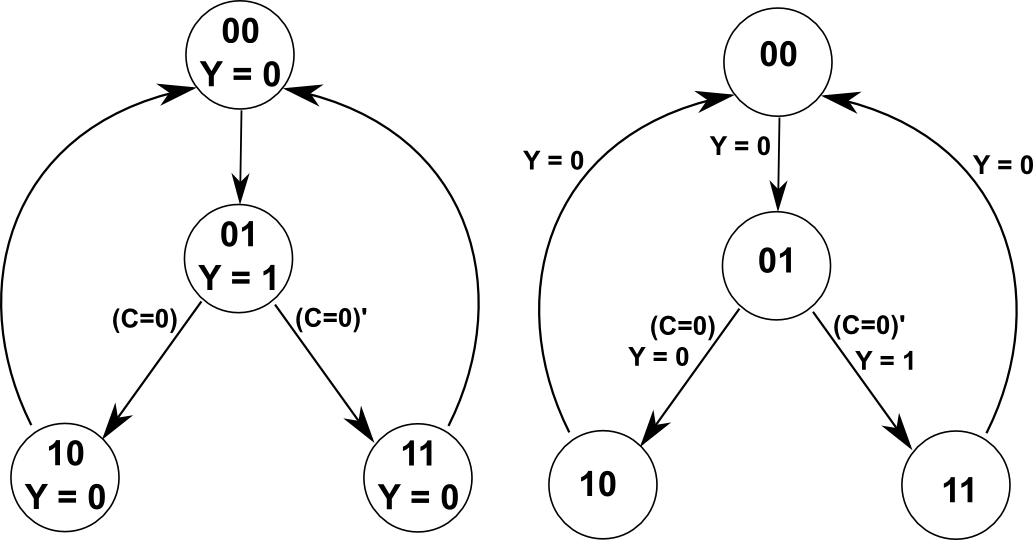
\includegraphics[height = 2.2in, width = 4in]{mealyvsmoore_6.png}
\end{frame}

%SEÇÃO == ANALISE
\section{Análise}
\begin{frame}
  \frametitle{Análise de circuitos sequenciais}
  Dado o circuito deseja-se obter a descrição precisa do mesmo, este processo é chamado de análise.
  \begin{block}{Etapas da análise}
   \begin{enumerate}
    \item Derive as \textbf{equações de excitação} do circuito de próximo estado (entrada dos FF).\pause
    \item Derive as \textbf{equações de próximo estado} substituindo as equações de excitação obtidas no passo anterior nas equações característica de cada FF.\pause
    \item Derive a \textbf{tabela do próximo estado} partindo das equações de próximo estado.\pause
    \item Derive as \textbf{equações de saída} do circuito.\pause
    \item Derive a tabela de saída para as equações de saída.\pause
    \item Faça o diagrama de estados utilizando a tabela de próximo estado e a tabela de saída.
   \end{enumerate}
  \end{block}
\end{frame}

%SUBSEÇÃO == EXEMPLO
\section{Exemplo}
\begin{frame}
  \frametitle{Exemplo}
  Aplicamos e detalhamos estes passos no exemplo a seguir.\\
  
  \textbf{Exemplo 1: Dado o circuito abaixo analise-o.}
   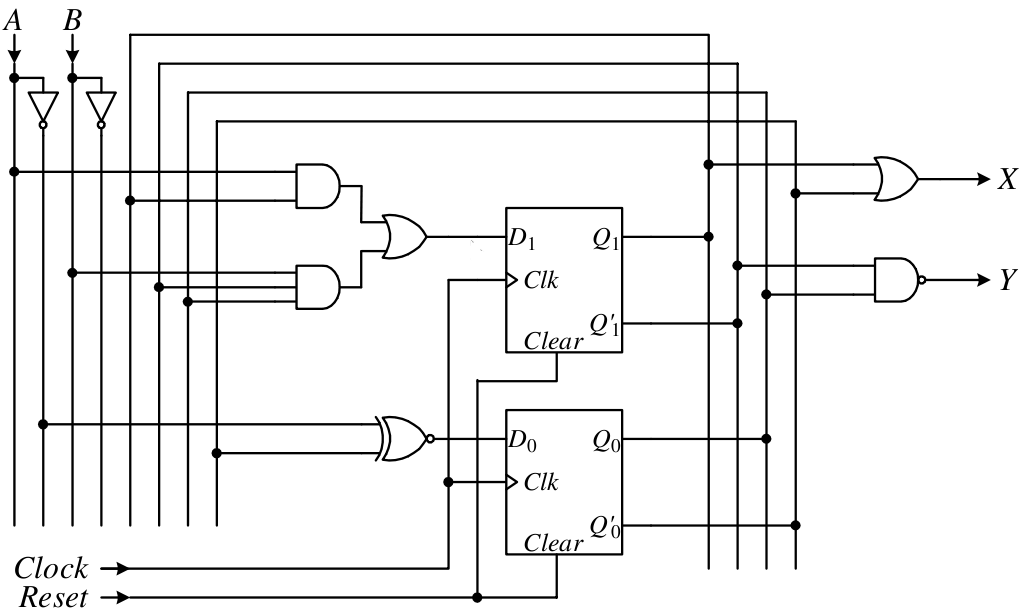
\includegraphics[height = 2.2in, width = 4in]{EXEMPLO_ANALISE_1.png}
\end{frame}

\begin{frame}
  \frametitle{Exemplo}
  \textbf{1 – Derive as equações de excitação}
  \begin{block}{\textbf{Equações de excitação}}
   As equações de excitação são extraídas do circuito combinacional, onde as saídas destes correspondem as entradas da memória dos estados em uma FSM. 
   Portanto temos uma equação para cada FF.
  \end{block}
\end{frame}

\begin{frame}
  \frametitle{Exemplo}
  \textbf{1 – Derive as equações de excitação}
   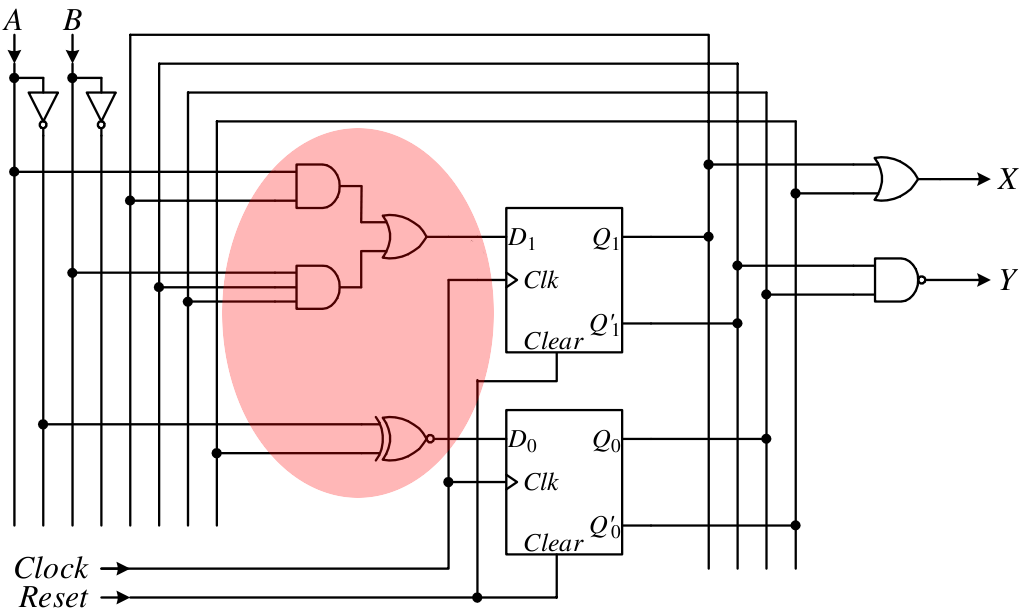
\includegraphics[height = 2.2in, width = 4in]{EXEMPLO_ANALISE_2.png}
\end{frame}

\begin{frame}
  \frametitle{Exemplo}
  \textbf{1 – Derive as equações de excitação}
  \begin{block}{\textbf{Equações de excitação do circuito}}
    \begin{enumerate}
     \item $ D_1 = AQ_1 + B\overline{Q_1}Q_0 $
     \item $ D_0 = (\overline{A}\odot\overline{Q_0}) = \overline{A}\overline{Q_0} + AQ_0 $
    \end{enumerate}
  \end{block}\pause
  Nada de mais, certo?
\end{frame}

\begin{frame}
  \frametitle{Exemplo}
  \textbf{2 – Derive as equações do próximo estado}
   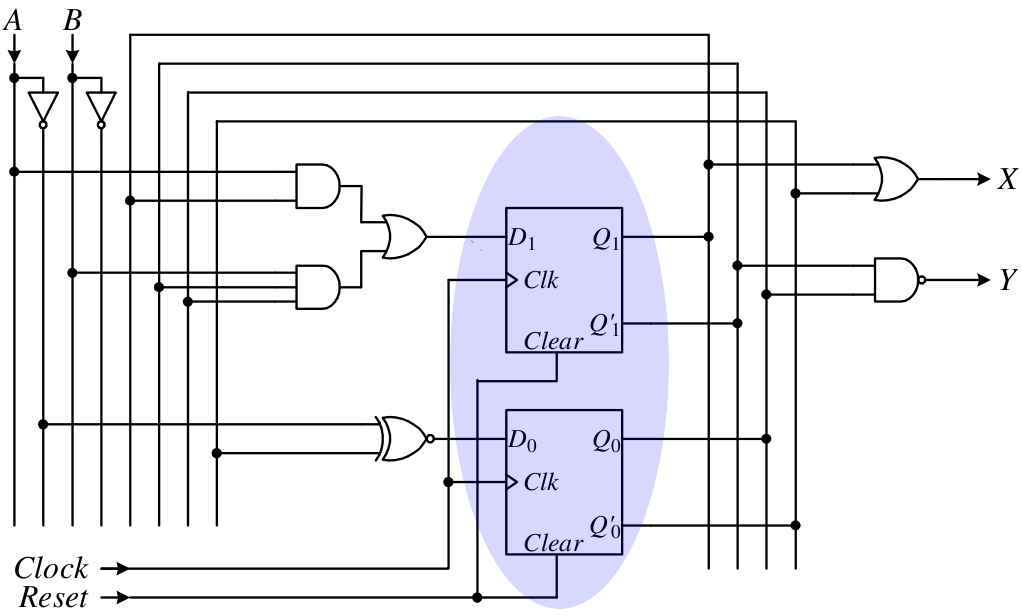
\includegraphics[height = 2.2in, width = 4in]{EXEMPLO_ANALISE_3.png}
\end{frame}

\begin{frame}
  \frametitle{Exemplo}
  \textbf{2 – Derive as equações do próximo estado}
  \begin{block}{\textbf{Equações do próximo estado}}
    De acordo com as entradas dos FFs e com o comportamento específico de cada FF (este é dado pela equação característica) a \textbf{equação do próximo estado} 
    especificará qual o próximo estado da FSM.
  \end{block}
\end{frame}

\begin{frame}
  \frametitle{Exemplo}
  \textbf{2 – Derive as equações do próximo estado}
  \begin{block}{\textbf{Equações do próximo estado do circuito}}
    A equação característica do Flip-Flop D é Q = D, logo temos
    \begin{enumerate}
     \item $ Q_{1next} = AQ_1 + B\overline{Q_1}Q_0 $
     \item $ Q_{0next} = (\overline{A}\odot\overline{Q_0}) = \overline{A}\overline{Q_0} + AQ_0 $
    \end{enumerate}
  \end{block}\pause
  Obs.: O Flip-flop D sem Enable é um caso especial, em geral ao se aplicar a equação característica a expressão $ Q \neq D $.
\end{frame}

\begin{frame}
  \frametitle{Exemplo}
  \textbf{3 – Tabela de próximo estado}
  \begin{block}{\textbf{Tabela de próximo estado}}
    A tabela do próximo estado é simplesmente uma tabela verdade derivada das equações do próximo estado. O valor destes próximos estados são obtidos simplesmente 
    substituindo o valor do estado atual e o valor da entrada na equação do próximo estado apropriada. 
  \end{block}
\end{frame}

\begin{frame}
  \frametitle{Exemplo}
  \textbf{3 – Tabela de próximo estado}

  \begin{center}
    \begin{tabular}{|c|c|}
      \hline
		      & Próximo estado\\
	Estado atual  & $Q_{1next}Q_{0next}$ \\
	 $Q_1Q_0$     & AB = \\
		  & \begin{tabular}{c|c|c|c} 00 & 01 & 10 & 11\\ \end{tabular} \\
      \hline
	00 \pause & \begin{tabular}{c|c|c|c} 01 \pause & 01 \pause & 00 \pause & 00 \pause  \\ \end{tabular} \\
      \hline
	01 \pause & \begin{tabular}{c|c|c|c} 00 \pause & 10 \pause & 01 \pause & 11 \pause  \\ \end{tabular} \\	
      \hline
	10 \pause & \begin{tabular}{c|c|c|c} 01 \pause & 01 \pause & 10 \pause & 10 \pause  \\ \end{tabular} \\
      \hline
	11 \pause & \begin{tabular}{c|c|c|c} 00 \pause & 00 \pause & 11 \pause & 11 \pause  \\ \end{tabular} \\
      \hline
  \end{tabular}
 \end{center}
\end{frame}

\begin{frame}
  \frametitle{Exemplo}
  \textbf{3 – Tabela de próximo estado}
  \begin{itemize}
   \item Estado atual: Coluna que contém todos os possíveis estados que a máquina pode atingir. Esta diretamente relacionada ao número de FF e em geral 
	 conseguimos preenchê-la logo de início.\pause
   \item Próximo estado: É a coluna que descreve qual será o próximo estado de acordo com as entradas. Repare que esta pode possuir n colunas onde, cada 
	 uma representa uma combinação das entradas.
  \end{itemize}
\end{frame}

\begin{frame}
  \frametitle{Exemplo}
  \textbf{4 – Equações de saída}
   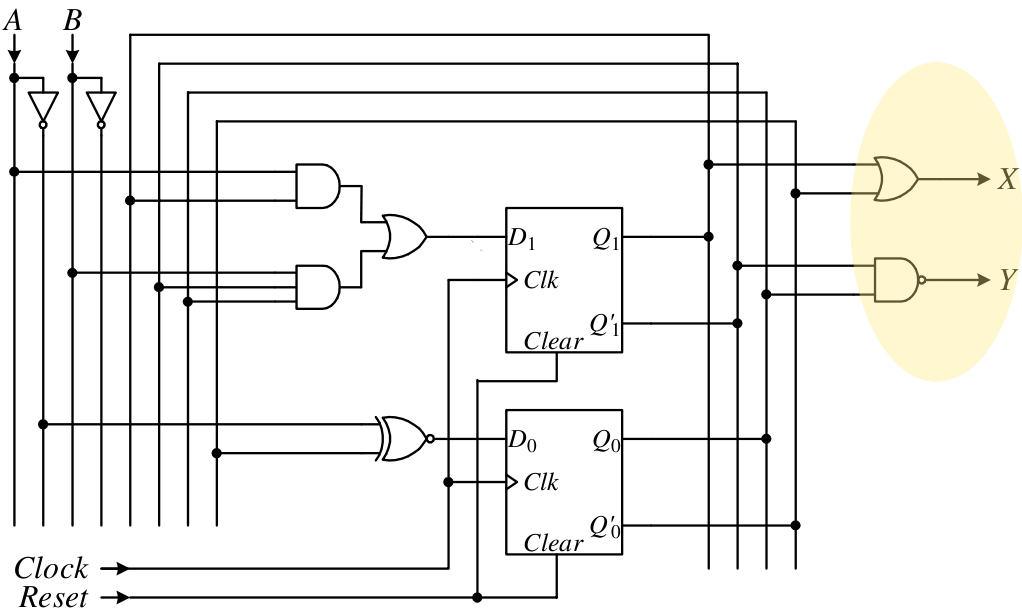
\includegraphics[height = 2.2in, width = 4in]{EXEMPLO_ANALISE_4.png}
\end{frame}

\begin{frame}
  \frametitle{Exemplo}
  \textbf{4 – Equações de saída}
   \begin{block}{\textbf{Equações de saída}}
    As equações de saída são derivadas do circuito combinacional da saída da FSM.
   \end{block}
\end{frame}

\begin{frame}
  \frametitle{Exemplo}
  \textbf{4 – Equações de saída}
   \begin{block}{\textbf{Equações de saída do circuito}}
     \begin{itemize}
      \item $X = Q_1 + \overline{Q_0}$
      \item $Y = \overline{(\overline{Q_1}Q_0)} = Q_1 + \overline{Q_0} $ 
     \end{itemize}
   \end{block}
\end{frame}

\begin{frame}
  \frametitle{Exemplo}
  \textbf{5 – Tabela de saída}
   \begin{block}{\textbf{Tabela de saída}}
    Como a tabela de próximo estado, a tabela de saída é uma tabela verdade que é derivada das equações de saída. 
   \end{block}
\end{frame}

\begin{frame}
  \frametitle{Exemplo}
  \textbf{5 – Tabela de saída}
  \begin{center}
    \begin{tabular}{|c|c|}
      \hline
	Estado atual & Saída \\
	$Q_1Q_0$ & $Q_{1next}Q_{0next}$ \\
	  & \begin{tabular}{cc} X & Y \\ \end{tabular} \\
      \hline
	00 \pause & \begin{tabular}{c|c} 1 \pause & 0 \pause\\ \end{tabular} \\
      \hline
	01 \pause & \begin{tabular}{c|c} 0 \pause & 0 \pause\\ \end{tabular} \\
      \hline
	10 \pause & \begin{tabular}{c|c} 1 \pause & 1 \pause\\ \end{tabular} \\
      \hline
	11 \pause & \begin{tabular}{c|c} 1 \pause & 1 \pause\\ \end{tabular} \\
      \hline
  \end{tabular}
 \end{center}
\end{frame}

\begin{frame}
  \frametitle{Exemplo}
  \textbf{6 – Diagrama de estados} \\
   O diagrama de estados dispensa apresentações formais. Segue a criação do diagrama de estados para o circuito do exemplo.
\end{frame}

\begin{frame}
 \frametitle{Exemplo}
 \textbf{6 – Diagrama de estados}
  \begin{itemize}
   \item Cada linha da tabela indica um estado, portanto nós teremos quatro estados para analisar.\pause 
   \item Temos duas entradas (A e B), que nós gera quatro possibilidades diferentes de entradas em para cada estado.\pause
   \item Começamos do estado inicial.
  \end{itemize}
\end{frame}

\begin{frame}
  \frametitle{Exemplo}
  \textbf{6 – Diagrama de estados}
  \begin{center}
   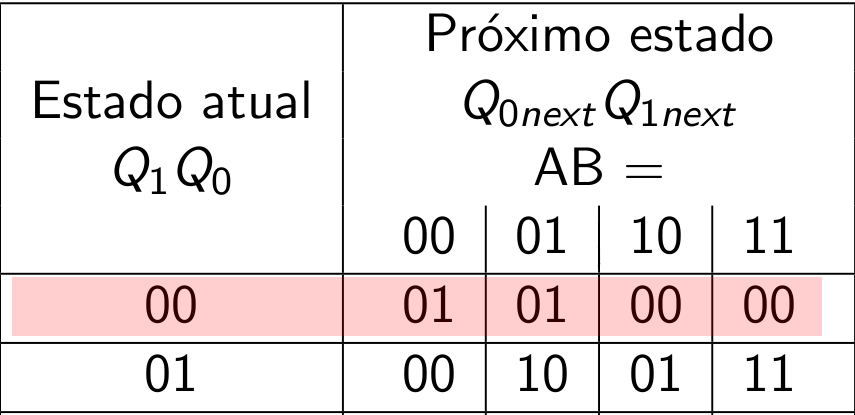
\includegraphics[height = 1.5in, width = 3.5in]{Diagrama_estado_tabela.png}
  \end{center}

  \begin{itemize}
   \item Analisando a tabela é possível notar que no estado 00 com a entrada A = 1, sempre leva ao mesmo estado independentemente 
	 de B. Logo temos AB = 1x em 00 leva a ele mesmo.\pause 
   \item Repare que se A = 0 no estado 00, teremos como próximo estado 01. Logo temos AB = 0x leva ao estado 01.
  \end{itemize} 
\end{frame}

\begin{frame}
  \frametitle{Exemplo}
  \textbf{6 – Diagrama de estados}
   \begin{center}
    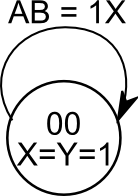
\includegraphics[height = 2.2in, width = 1.7in]{Diagrama_de_estado_ex1.png}
   \end{center}
\end{frame}

\begin{frame}
  \frametitle{Exemplo}
  \textbf{6 – Diagrama de estados}
   \begin{center}
    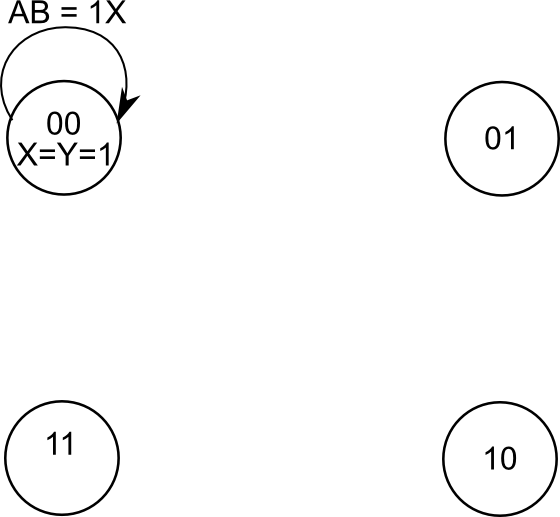
\includegraphics[height = 2.2in, width = 2.5in]{Diagrama_de_estado_ex2.png}
   \end{center}
\end{frame}

\begin{frame}
  \frametitle{Exemplo}
  \textbf{6 – Diagrama de estados}
   \begin{center}
    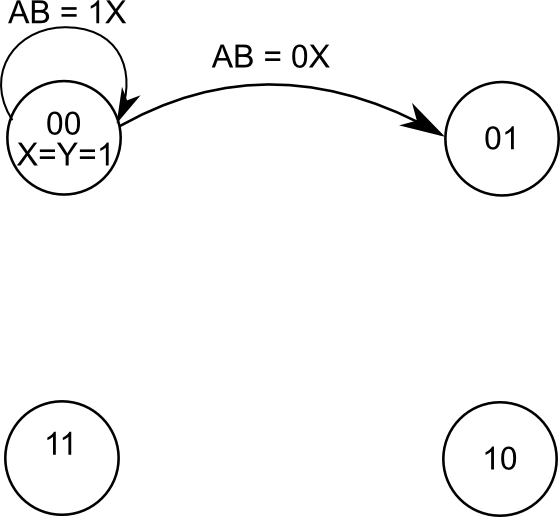
\includegraphics[height = 2.2in, width = 2.5in]{Diagrama_de_estado_ex3.png}
   \end{center}
\end{frame}

\begin{frame}
  \frametitle{Exemplo}
  \textbf{6 – Diagrama de estados}
  \begin{center}
   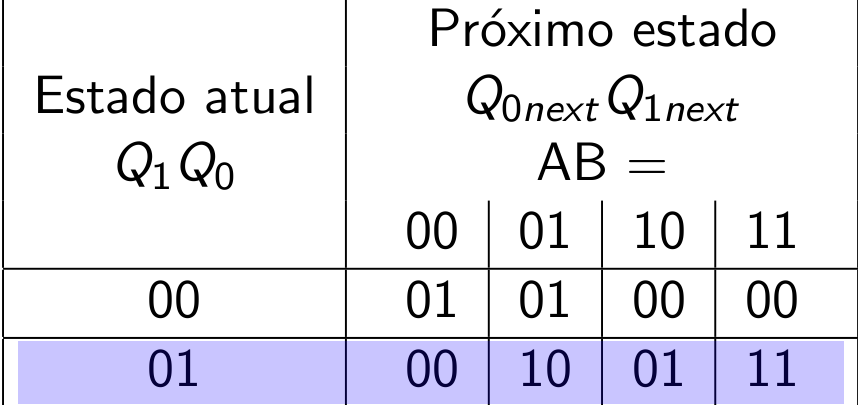
\includegraphics[height = 1in, width = 2.7in]{Diagrama_estado_tabela_2.png}
  \end{center}

  \begin{itemize}
   \item Agora analisamos a segunda linha da tabela correspondente ao estado 01. E logo de início notamos que as saídas X e Y neste estado são iguais a 0.\pause
   \item Se AB = 10 então o circuito permanecerá em 01. \pause
   \item Se AB = 11 então o circuito irá para o estado 11. \pause
   \item Se AB = 00 então o circuito irá para o estado 00. \pause
   \item Se AB = 01 então o circuito irá para o estado 10. 
  \end{itemize} 
\end{frame}

\begin{frame}
  \frametitle{Exemplo}
  \textbf{6 – Diagrama de estados}
   \begin{center}
    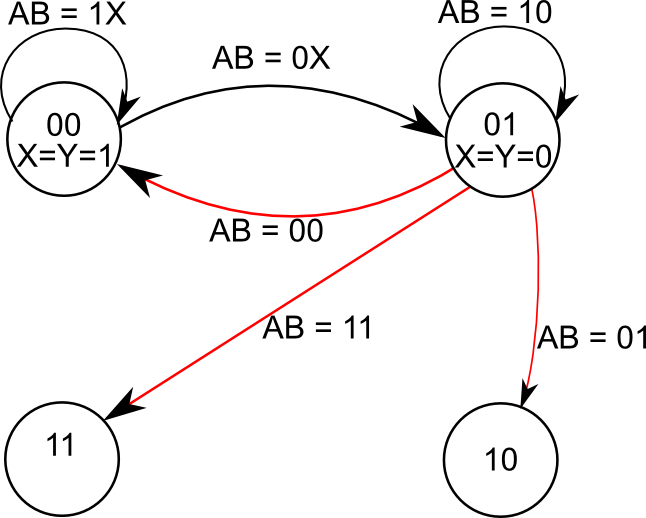
\includegraphics[height = 2.2in, width = 2.5in]{Diagrama_de_estado_ex4.png}
   \end{center}
\end{frame}

\begin{frame}
  \frametitle{Exemplo}
  \textbf{6 – Diagrama de estados}
  \begin{center}
   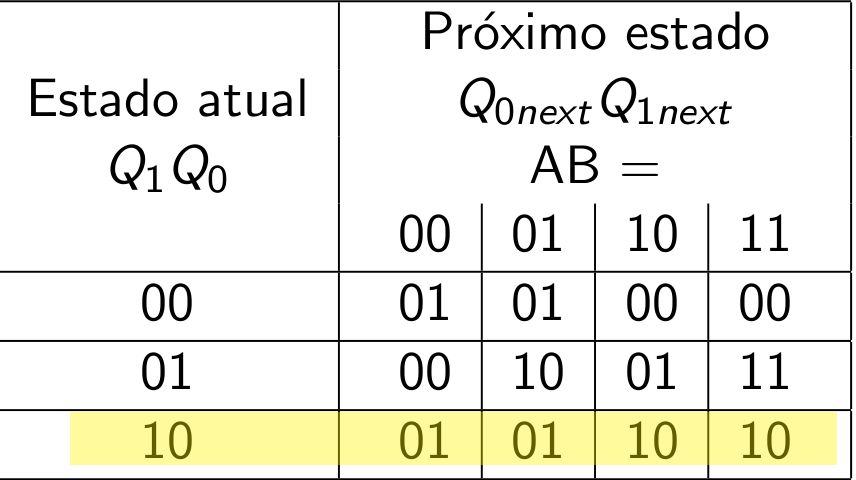
\includegraphics[height = 1in, width = 2.7in]{Diagrama_estado_tabela_3.png}
  \end{center}

  \begin{itemize}
   \item O resto da montagem do diagrama segue o mesmo procedimento. 
  \end{itemize} 
\end{frame}

\begin{frame}
  \frametitle{Exemplo}
  \textbf{6 – Diagrama de estados}
  \begin{center}
   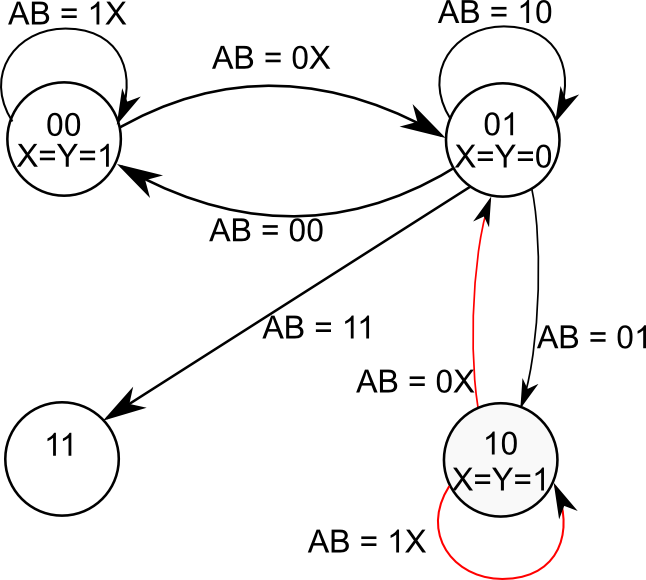
\includegraphics[height = 2.2in, width = 2.5in]{Diagrama_de_estado_ex5.png}
  \end{center}
\end{frame}

\begin{frame}
  \frametitle{Exemplo}
  \textbf{6 – Diagrama de estados}
  \begin{center}
   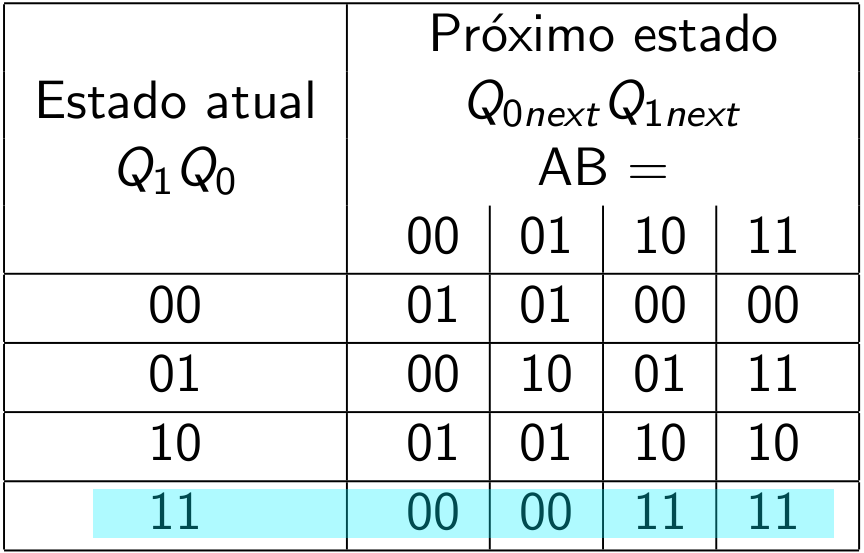
\includegraphics[height = 1in, width = 3in]{Diagrama_estado_tabela_4.png}
  \end{center}
\end{frame}

\begin{frame}
  \frametitle{Exemplo}
  \textbf{6 – Diagrama de estados}
  \begin{center}
   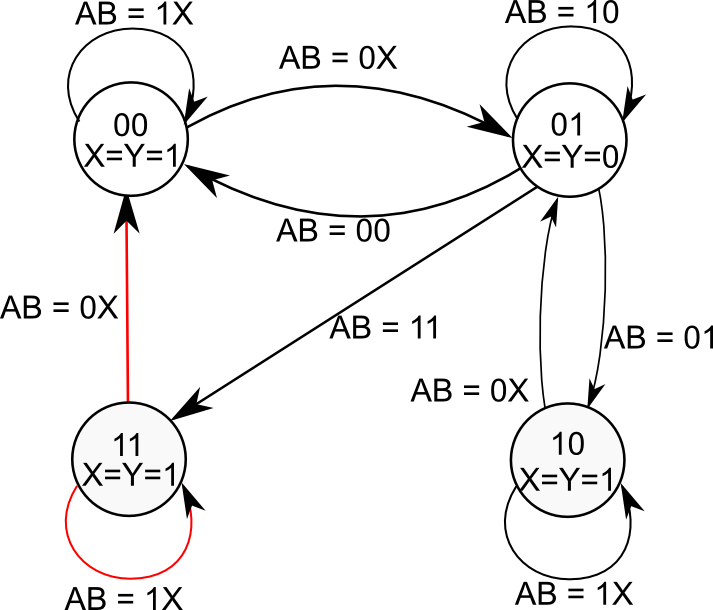
\includegraphics[height = 2.2in, width = 2.5in]{Diagrama_de_estado_ex6.png}
  \end{center}
\end{frame}

\begin{frame}
  \frametitle{Exemplo}
  \textbf{6 – Diagrama de estados}
  \begin{center}
   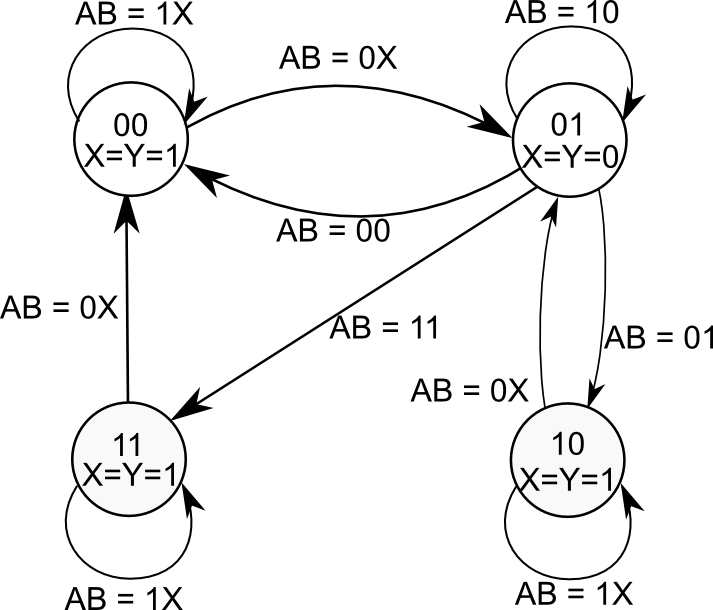
\includegraphics[height = 2.2in, width = 2.5in]{Diagrama_de_estado_ex7.png}
  \end{center}
\end{frame}

%SEÇÃO == BIBLIOGRAFIA
\section{Bibliografia}
\begin{frame}
 \frametitle{Referências bibliográficas}
 \begin{itemize}
  \item Digital Logic and Microprocessor Design With VHDL – Enoch O . Hwang
  \item Digital Design Principles And Practices - Wakerly
 \end{itemize}
\end{frame}

%SEÇÃO == COLABORADORES
\section{Colaboradores}
\begin{frame}
 \frametitle{Colaboradores}
 \begin{enumerate}
  \item Rodrigo Siqueira de Melo
 \end{enumerate}
\end{frame}

\end{document}
